\section{Consuntivazione}

\subsection{Milestones:}
\begin{itemize}
    \item Release versione 0.0.3 (Completa al: 100\%)
\end{itemize}

\subsection{Attività svolte}


\begin{table}[ht]
    \begin{tabularx}{\textwidth}{X l l}
        
        \rowcolor{gray!30} \textbf{Attività} & \textbf{Stato} & \textbf{Ruolo}\\
        
        \hline
        prima stesura del glossario dei termini & completato & Analista\\
        prima bozza vincoli di progettazione & completato & Analista\\
        prima bozza obiettivi di prodotto & completato & Analista\\
        prima bozza caratteristiche degli utenti & completato & Analista\\
        prima bozza caratteristiche del prodotto & completato & Analista\\
        prima bozza descrizione attori & completato & Analista\\
        aggiornato registro modifiche per il rilascio & completato & Analista e Verificatore\\
    \end{tabularx}
    \caption{Lista delle attività svolte durante lo sprint}
\end{table}


\begin{table}[ht]
    \begin{tabularx}{\linewidth}{X|rrrrrrr}
    \rowcolor{gray!30}& Re & Amm & An & Pro & Prog & Ver & tot \\
    \hline
    Bonavigo Michele                        & 0 & 0 & 0 & 0 & 0 & 2,9  & 2,9 \\
    \rowcolor{gray!10}Casarotto Mattia      & 3,5 & 0 & 0 & 0 & 0 & 0  & 3,5 \\
    Massarenti Alessandro                   & 0 & 0 & 2,4 & 0 & 0 & 1,2  & 3,6 \\
    \rowcolor{gray!10}Peron Samuel          & 0 & 0 & 2,5 & 0 & 0 & 0 & 2,5 \\
    Pierobon Luca                           & 0 & 5 & 0 & 0 & 0 & 0,1 & 5,1 \\
    \rowcolor{gray!10}Romano Davide         & 0 & 0 & 3,1 & 0 & 0 & 0 & 3,1 \\
    Zarantonello Giorgio                    & 0 & 0 & 2,5 & 0 & 0 & 0 & 2,5 \\
    \hline                                  & 3,5 & 5 & 10,5 & 0 & 0 & 4,2 & 
    \end{tabularx}
    \caption{\label{ruoli-persone}Spartizione dei ruoli e ore svolte durante lo sprint}
\end{table}

\begin{center}
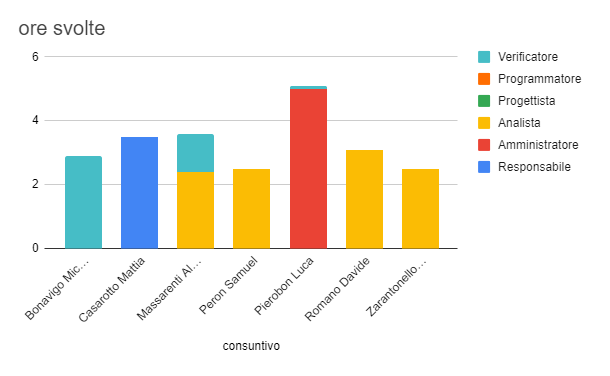
\includegraphics[width=12cm]{img/ore-usate.png}
\end{center}

\begin{table}[ht]
    \begin{tabularx}{\linewidth}{X|l|l}
    \rowcolor{gray!30}& Ore & Costo \\
    \hline
    
    Responsabile & 3,5 & € 105,00 \\
    \rowcolor{gray!10}Amministratore & 5 & € 100,00 \\
    Analista & 10,5 & € 262,50 \\
    \rowcolor{gray!10}Progettista & 0 & € 0,00 \\
    Programmatore & 0 & € 0,00 \\
    \rowcolor{gray!10}Verificatore & 4,2 &€ 63,00 \\
    totale & 23,2 & € 530,50 \\
    \end{tabularx}
    \caption{\label{costi-ruolo}Spartizione dei ruoli e ore svolte durante lo sprint}
\end{table}


Avendo quindi consumato €530,50\footnote{Si veda tabella \ref{costi-ruolo}} del budget durante questo sprint, rimangono ancora a disposizione € 13002,75 per gli sprint seguenti.

\subsection{Difficoltà e problemi di sprint}

Alcune questioni sono risultate durante questo sprint:

\begin{itemize}
    \item Comprendere a fondo i bisogni del capitolato.
\end{itemize}

Queste verranno discusse in sede di preparazione del prossimo sprint.
